\documentclass{article}
\usepackage{amsmath, amsthm, amssymb}
\usepackage{tikz}
\usepackage{array}
\usepackage{mathtools}
\usepackage{graphicx}

\begin{document}
\section*{\huge Homework Sheet 2}
\begin{flushright}
   \textbf{Author: Abdullah Oğuz Topçuoğlu \& Yousef Mostafa Farouk}
\end{flushright}

% Task 1 (4 points) Let Σ = {a, b}. Investigate the following two languages on whether they are
% DFA languages or not. Prove your answers!
% 1. (2 points) L1 = { w ∈ Σ
% ∗
% | #a(w) mod 2 = #b(w) mod 2 }
% 2. (2 points) L2 = { w ∈ Σ
% ∗
% | #a(w) mod k = #b(w) mod ` },
% where k and ` are some fixed given natural numbers bigger than 1 (imagine, say, k = 3
% and ` = 5.)
% Here #x(w) for x ∈ Σ and w ∈ Σ
% ? denotes the number of occurences of the letter x in w.
% Task 2 (4 points) Let Σ = {0, 1}. For x = xn−1xn−2 · · · x1x0 let hxi2 =
% P
% 0≤i<n xi2
% i be the number
% denoted by string x in the binary system. Investigate the following two languages on whether
% they are DFA languages or not. Prove your answers!
% 1. (2 points) L3 = { x ∈ Σ
% ∗
% | hxi2 mod 3 = 0 }
% 2. (2 points) L4 = { x ∈ Σ
% ∗
% | hxi2 is not a perfect square }
% Task 3 (6 points) Let Σ = {a, b}.
% 1. (2 points) Design an NFA that accepts exactly all words in Σ
% ∗
% for which the 3rd-last
% letter is an a. Try to make your NFA have few states.
% 2. (2 points) Design a DFA that accepts exactly all words in Σ
% ∗
% for which the 3rd-last
% letter is an a. Try to make your DFA have few states.
% 3. (2 points) If “4th-last” were replaced by “kth-last” for some fixed integer k ≥ 1, how
% would your constructions from the parts above and corresponding numbers of states
% change (no proof needed)?
% Task 4 (2 points)
% Design a DFA that recognizes the language
% S = { a
% n
% | n > 1600 and n is a leap year in the Gregorian Calendar }.

\section*{Problem 4}
\begin{figure}[h!]
  \centering
  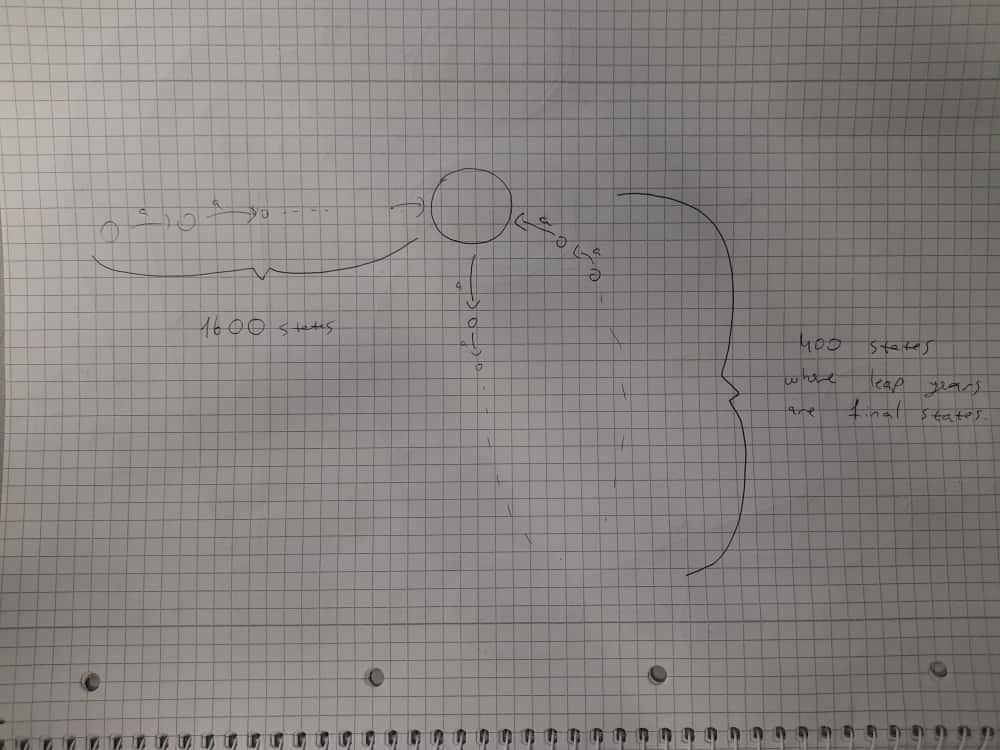
\includegraphics[width=0.9\textwidth]{4.jpeg}
  \caption{leap year dfa}
\end{figure}

We can design a DFA with 2000 states. The first 1600 states will be just a chain of states from 0 to 1599. After that we have a looping 400 states where leap years are final states.
The chain part is for "\(>\) 1600" condition in the question. And the looping 400 states part is for detecting the leap years.

\end{document}